\documentclass[12pt,a4paper]{article}

\usepackage[a4paper,margin=1in]{geometry}
\usepackage{fontspec}
\usepackage{ctex}
\usepackage{amsmath,amssymb}
\usepackage{graphicx}
\usepackage{booktabs}
\usepackage{array}
\usepackage{longtable}
\usepackage{caption}
\usepackage{float}
\usepackage{setspace}
\usepackage{fancyhdr}
\usepackage{hyperref}
\usepackage{xcolor}
\usepackage{enumitem}
\usepackage{listings}
\renewcommand{\tablename}{Table}

\setcounter{tocdepth}{2}
\setmainfont{Noto Serif}
\setmonofont{DejaVu Sans Mono}
\onehalfspacing
\setlength{\parindent}{2em}
\setlength{\parskip}{0.4em}
\pagestyle{fancy}
\fancyhf{}
\fancyfoot[C]{\thepage}
\renewcommand{\headrulewidth}{0pt}
\hypersetup{colorlinks=true,linkcolor=blue,urlcolor=blue,citecolor=blue}
\lstset{basicstyle=\ttfamily\small,breaklines=true,frame=single,columns=fullflexible,showstringspaces=false}

\newcommand{\HomeworkTitle}{Computational Physics Hw\_4}
\newcommand{\StudentID}{2024141230044}
\newcommand{\StudentName}{Fanyi}

\begin{document}

\begin{center}
    {\LARGE \textbf{\HomeworkTitle}}\\[1.2em]
    {\large Student ID: \StudentID}\\[0.5em]
    {\large Name: \StudentName}
\end{center}

\vspace{0.5em}
\noindent\rule{\textwidth}{0.8pt}
\vspace{0.5em}

\section*{Problem 2}

For the function
\[
    f(x)=(x-1)^{10},
\]
compare three evaluation methods:
\begin{enumerate}[leftmargin=2.5em]
    \item direct evaluation of $(x-1)^{10}$,
    \item direct evaluation of the expanded polynomial,
    \item Horner's method for the expanded polynomial.
\end{enumerate}
The calculations are carried out in single precision (float), double precision (double), and quad precision (\texttt{\_\_float128}). The interval is zoomed to $x\in[0.7,1.3]$, and the relative error distribution of the expansion is examined. Finally, Horner's method is compared with the naive expansion and the numerical behavior is explained.

\newpage
\tableofcontents
\newpage

\section{Algorithm Principle}

\subsection{Three equivalent formulas}
For the same mathematical function,
\[
    f(x)=(x-1)^{10},
\]
we compare the following three implementations.

\paragraph{Direct form.}
Compute
\[
    f(x)=(x-1)^{10}
\]
by first forming $x-1$, then multiplying ten times.

\paragraph{Expanded polynomial.}
Use the binomial expansion
\[
\begin{aligned}
(x-1)^{10}={}&x^{10}-10x^9+45x^8-120x^7+210x^6 \\
&-252x^5+210x^4-120x^3+45x^2-10x+1.
\end{aligned}
\]
This form is algebraically correct, but near $x=1$ the individual terms are large and nearly cancel, so it is sensitive to roundoff.

\paragraph{Horner form.}
Rewrite the same polynomial as
\[
\begin{aligned}
f(x)=&((((((((((x-10)x+45)x-120)x+210)x-252) \\
&\qquad x+210)x-120)x+45)x-10)x+1.
\end{aligned}
\]
Horner's method reduces the number of multiplications and avoids explicitly computing high powers. It is usually more stable than the naive expanded form, although it still evaluates the same cancellation-prone polynomial.

\subsection{Reference value and relative error}
The program uses quad precision direct evaluation as the reference value:
\[
    f_{\mathrm{ref}}(x)=\texttt{direct\_q}(x).
\]
For an approximation $f_{\mathrm{approx}}(x)$, the relative error is
\[
    \mathrm{relerr}(x)=\left|\frac{f_{\mathrm{approx}}(x)-f_{\mathrm{ref}}(x)}{f_{\mathrm{ref}}(x)}\right|.
\]
At $x=1$, the exact value is $0$, so the relative error is undefined; the program writes \texttt{nan} at that point.

\section{Program Code}

\begin{lstlisting}[language=C]
#include <stdio.h>
#include <stdlib.h>
#include <math.h>
#include <quadmath.h>

typedef __float128 quad_t;

static const int C[11] = {1, -10, 45, -120, 210, -252, 210, -120, 45, -10, 1};

static float direct_f(float x) {
    float t = x - 1.0f;
    float y = 1.0f;
    for (int i = 0; i < 10; ++i) y *= t;
    return y;
}

static double direct_d(double x) {
    double t = x - 1.0;
    double y = 1.0;
    for (int i = 0; i < 10; ++i) y *= t;
    return y;
}

static quad_t direct_q(quad_t x) {
    quad_t t = x - (quad_t)1.0;
    quad_t y = (quad_t)1.0;
    for (int i = 0; i < 10; ++i) y *= t;
    return y;
}

static float expand_f(float x) {
    float p[11];
    p[0] = 1.0f;
    for (int i = 1; i <= 10; ++i) p[i] = p[i - 1] * x;
    float y = 0.0f;
    for (int i = 0; i <= 10; ++i) y += (float)C[i] * p[10 - i];
    return y;
}

static double expand_d(double x) {
    double p[11];
    p[0] = 1.0;
    for (int i = 1; i <= 10; ++i) p[i] = p[i - 1] * x;
    double y = 0.0;
    for (int i = 0; i <= 10; ++i) y += (double)C[i] * p[10 - i];
    return y;
}

static quad_t expand_q(quad_t x) {
    quad_t p[11];
    p[0] = (quad_t)1.0;
    for (int i = 1; i <= 10; ++i) p[i] = p[i - 1] * x;
    quad_t y = (quad_t)0.0;
    for (int i = 0; i <= 10; ++i) y += (quad_t)C[i] * p[10 - i];
    return y;
}

static float horner_f(float x) {
    float y = (float)C[0];
    for (int i = 1; i <= 10; ++i) y = y * x + (float)C[i];
    return y;
}

static double horner_d(double x) {
    double y = (double)C[0];
    for (int i = 1; i <= 10; ++i) y = y * x + (double)C[i];
    return y;
}

static quad_t horner_q(quad_t x) {
    quad_t y = (quad_t)C[0];
    for (int i = 1; i <= 10; ++i) y = y * x + (quad_t)C[i];
    return y;
}
\end{lstlisting}

\section{Numerical Results}

The program samples 6001 equally spaced points on $[0.7,1.3]$. It outputs two CSV files:
\begin{itemize}[leftmargin=2.5em]
    \item \texttt{values.csv}: the computed function values for all methods;
    \item \texttt{relerr.csv}: the relative errors against quad direct evaluation.
\end{itemize}

\subsection{Zoomed function plots}
Figures \ref{fig:valf}--\ref{fig:valq} compare the three formulas in float, double, and quad precision.

\begin{figure}[H]
    \centering
    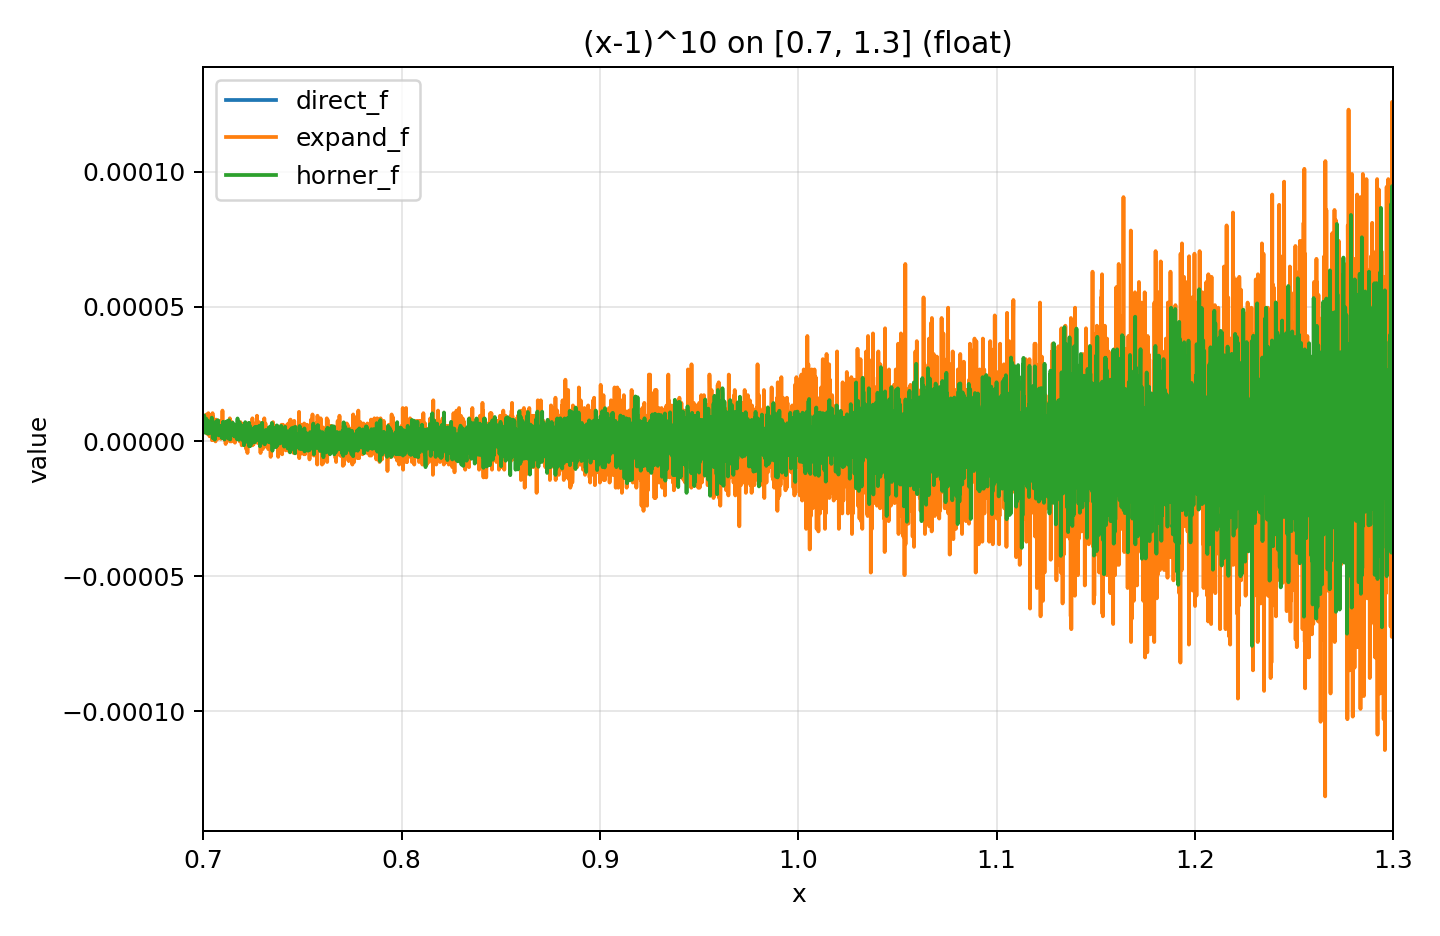
\includegraphics[width=0.88\textwidth]{values_float.png}
    \caption{Function values on $[0.7,1.3]$ in float precision.}
    \label{fig:valf}
\end{figure}

\begin{figure}[H]
    \centering
    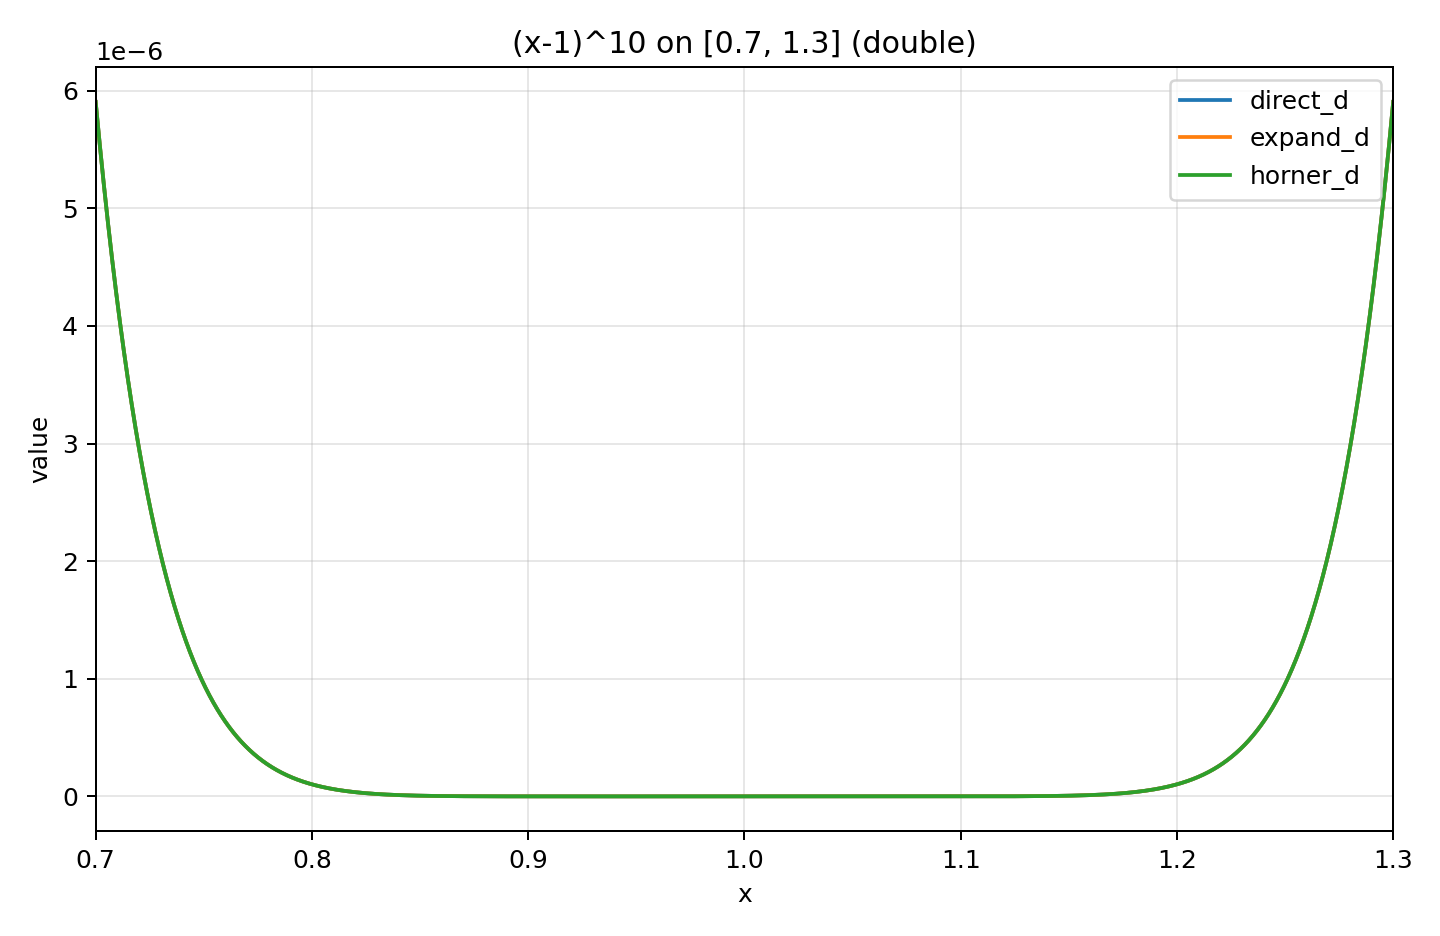
\includegraphics[width=0.88\textwidth]{values_double.png}
    \caption{Function values on $[0.7,1.3]$ in double precision.}
    \label{fig:vald}
\end{figure}

\begin{figure}[H]
    \centering
    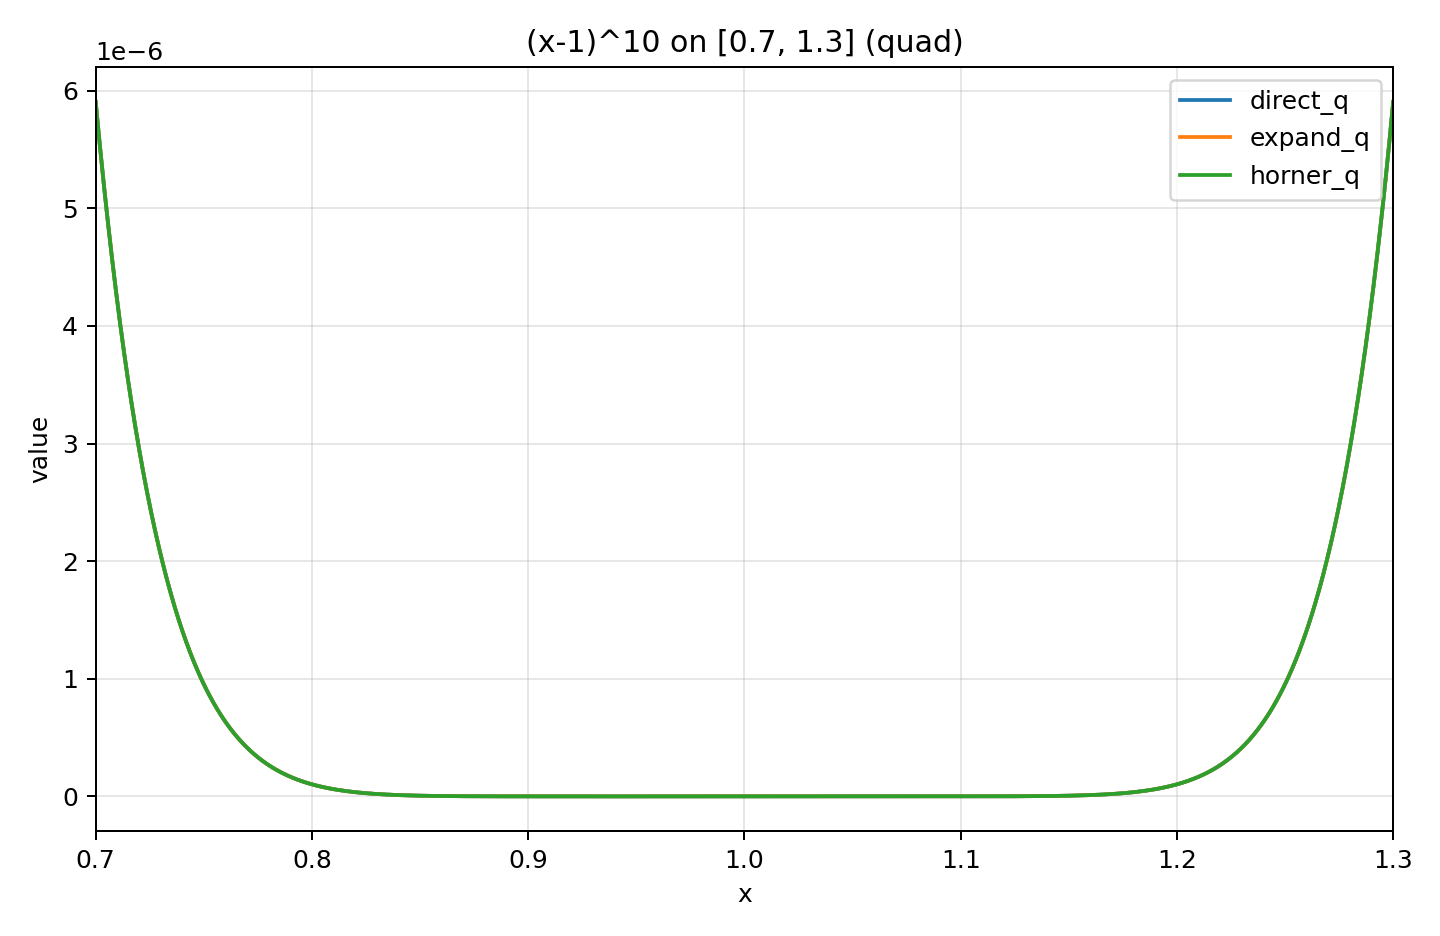
\includegraphics[width=0.88\textwidth]{values_quad.png}
    \caption{Function values on $[0.7,1.3]$ in quad precision.}
    \label{fig:valq}
\end{figure}

From the plots, the direct evaluation remains smooth and consistent across precisions. By contrast, the naive expanded form oscillates strongly near $x=1$, especially in float and double precision. Horner's method improves the expanded evaluation, but it still shows visible deviation near $x=1$ because the underlying cancellation problem is still present.

\subsection{Relative error distribution}
Figures \ref{fig:errf}--\ref{fig:errq} show the relative-error distributions. Since the exact value becomes extremely small near $x=1$, even tiny absolute perturbations can produce enormous relative errors.

\begin{figure}[H]
    \centering
    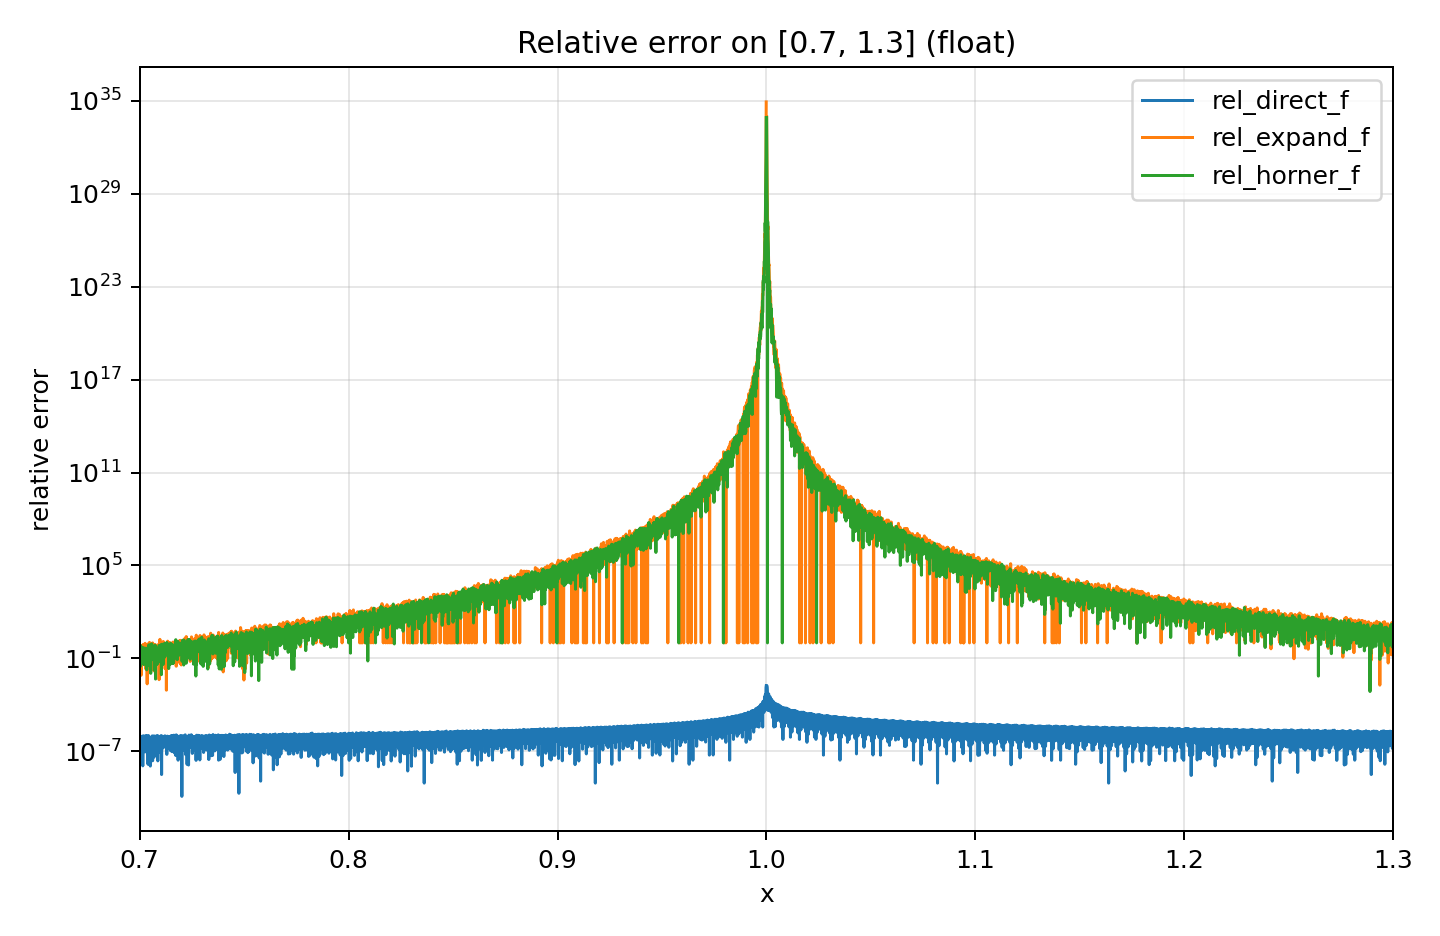
\includegraphics[width=0.88\textwidth]{relerr_float.png}
    \caption{Relative error in float precision.}
    \label{fig:errf}
\end{figure}

\begin{figure}[H]
    \centering
    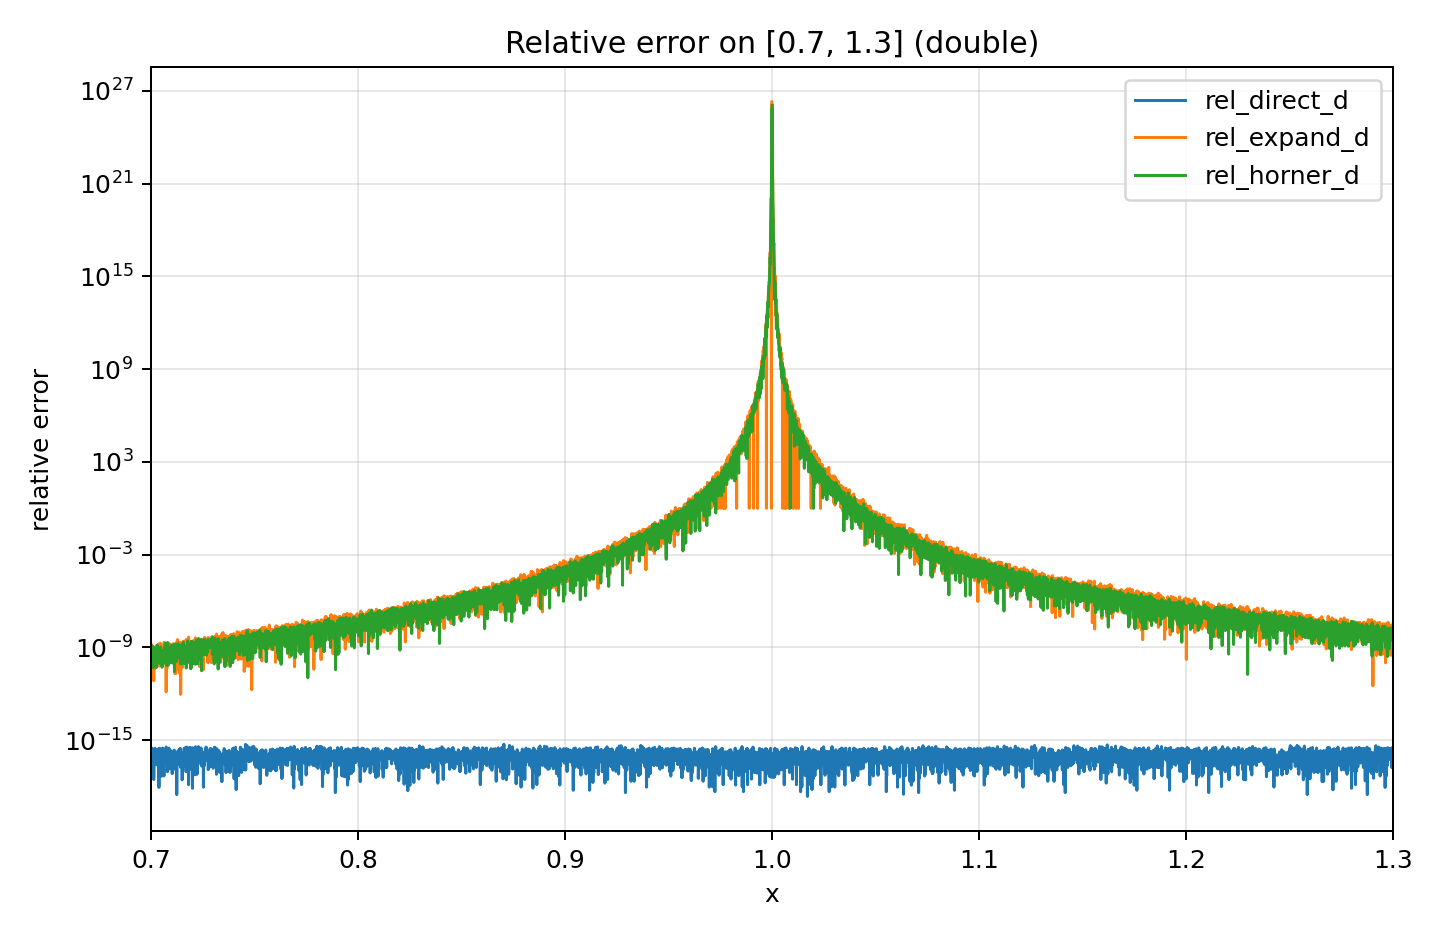
\includegraphics[width=0.88\textwidth]{relerr_double.png}
    \caption{Relative error in double precision.}
    \label{fig:errd}
\end{figure}

\begin{figure}[H]
    \centering
    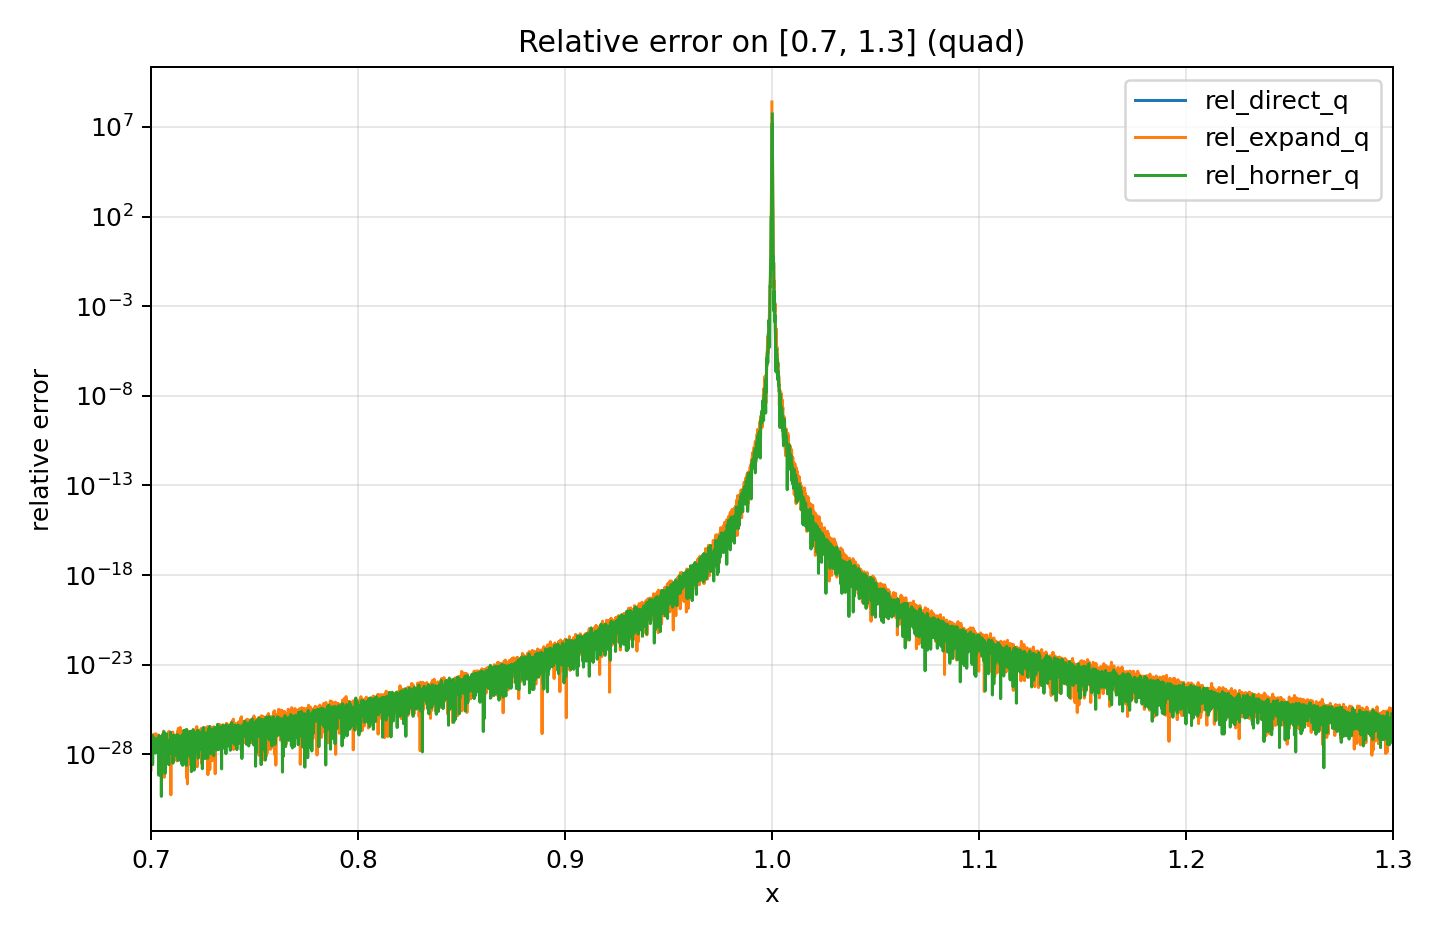
\includegraphics[width=0.88\textwidth]{relerr_quad.png}
    \caption{Relative error in quad precision.}
    \label{fig:errq}
\end{figure}

\subsection{Representative data points}
A few representative points illustrate the behavior more clearly.

\begin{table}[H]
\centering
\caption{Representative double-precision results.}
\begin{tabular}{>{\raggedleft\arraybackslash}p{1.4cm} >{\raggedleft\arraybackslash}p{3cm} >{\raggedleft\arraybackslash}p{3cm} >{\raggedleft\arraybackslash}p{3cm}}
\toprule
$x$ & direct\_d & expand\_d & horner\_d \\
\midrule
0.90   & $1.000000\times10^{-10}$ & $1.000160\times10^{-10}$ & $1.000179\times10^{-10}$ \\
0.99   & $1.000000\times10^{-20}$ & $1.953993\times10^{-14}$ & $3.219647\times10^{-15}$ \\
0.9999 & $1.000000\times10^{-40}$ & $-1.953993\times10^{-14}$ & $-5.995204\times10^{-15}$ \\
1.0001 & $1.000000\times10^{-40}$ & $1.243450\times10^{-14}$ & $-1.154632\times10^{-14}$ \\
1.01   & $1.000000\times10^{-20}$ & $5.151435\times10^{-14}$ & $-8.881784\times10^{-16}$ \\
1.10   & $1.000000\times10^{-10}$ & $1.000089\times10^{-10}$ & $1.000238\times10^{-10}$ \\
\bottomrule
\end{tabular}
\end{table}

\begin{table}[H]
\centering
\caption{Representative relative errors in double precision.}
\begin{tabular}{>{\raggedleft\arraybackslash}p{1.4cm} >{\raggedleft\arraybackslash}p{3cm} >{\raggedleft\arraybackslash}p{3cm} >{\raggedleft\arraybackslash}p{3cm}}
\toprule
$x$ & relerr(direct\_d) & relerr(expand\_d) & relerr(horner\_d) \\
\midrule
0.90   & $6.96\times10^{-17}$ & $1.60\times10^{-4}$ & $1.79\times10^{-4}$ \\
0.99   & $2.42\times10^{-16}$ & $1.95\times10^{6}$  & $3.22\times10^{5}$ \\
0.9999 & $7.85\times10^{-17}$ & $1.95\times10^{26}$ & $5.99\times10^{25}$ \\
1.0001 & $7.85\times10^{-17}$ & $1.24\times10^{26}$ & $1.15\times10^{26}$ \\
1.01   & $2.42\times10^{-16}$ & $5.15\times10^{6}$  & $8.88\times10^{4}$ \\
1.10   & $5.66\times10^{-17}$ & $8.89\times10^{-5}$ & $2.38\times10^{-4}$ \\
\bottomrule
\end{tabular}
\end{table}

These tables show three main facts:
\begin{enumerate}[leftmargin=2.5em]
    \item The direct form is the most reliable, because it works with the small quantity $x-1$ from the start.
    \item The expanded polynomial is extremely unstable near $x=1$, where large terms cancel to produce a tiny exact value.
    \item Horner's method is clearly better than naive expansion, but it does not completely remove the cancellation built into the expanded polynomial.
\end{enumerate}

\section{Discussion}

\subsection{Why does the expansion fail near $x=1$?}
When $x\approx1$, each term in the expanded polynomial,
\[
    x^{10},\ -10x^9,\ 45x^8,\ \dots,\ -10x,\ 1,
\]
is individually of order $1$, but their final sum is of order $|x-1|^{10}$, which can be as small as $10^{-40}$ for $x=1\pm10^{-4}$. Thus the result is obtained by subtracting several nearly equal numbers, and the final tiny value is easily buried by roundoff. This is a典型的 catastrophic cancellation example.

\subsection{Why is Horner's method better?}
Horner's method evaluates the polynomial with fewer arithmetic operations and without forming every power separately. Therefore it reduces the accumulation of roundoff and repeated recomputation. This is why Horner's curve is usually closer to the direct result than the naive expanded curve. However, Horner's method still evaluates the expanded polynomial itself, so it cannot fully avoid the loss of significance near $x=1$.

\subsection{What is the best formula?}
For this problem, the best practical formula is the direct one:
\[
    (x-1)^{10}.
\]
It aligns the computation with the true scale of the answer. The closer the algebraic form is to the numerical structure of the result, the more stable the computation tends to be.

\section{Conclusion}

The numerical experiment satisfies all requested tasks for Problem 2:
\begin{itemize}[leftmargin=2.5em]
    \item the function was computed in single, double, and quad precision;
    \item the plots were zoomed to $x\in[0.7,1.3]$;
    \item the relative error distribution was drawn;
    \item Horner's method was implemented and compared with the direct expansion.
\end{itemize}

The conclusion is clear: near $x=1$, the expanded polynomial suffers severe cancellation, producing extremely large relative errors. Horner's method alleviates the problem but does not eliminate it. Direct evaluation of $(x-1)^{10}$ is the most numerically stable method.

\end{document}
